\documentclass[]{article}
\usepackage{graphicx}
\usepackage{float}
\usepackage{amsmath}
%\usepackage[]{hyperref}
% Title Page
\title{Lab 5}
\author{
	Alex Taglieri
	\\
	Andrew Kacherski
	}

\begin{document}
\maketitle
\newpage
\
\raggedright


\pagenumbering{arabic}
\section{Introduction and Background}

This lab shows the effects of damping on the a driven mass-spring system.

The general formula for the oscillation of a damped mass-spring system is given by the following equation:


\begin{equation}\label{uncertaintyLong}
x(t) = Ae^{\frac{-\gamma t}{2}}cos(\omega_d t + \phi)
\end{equation}

where $A$ is the amplitude, $\gamma$ is the damping ratio and can be found using the expression  $\gamma = \frac{b}{m}$ (where $b$ is the damping coefficient and $m$ is the mass), $t$ is time, $\omega_d$ is the damped frequency, and $\phi$ is the phase shift.

$\omega_d$ can be calculated using $k$, $m$, and $b$ (where $k$ is the spring constant):

\begin{equation}
	\omega_d = \sqrt{\frac{k}{m} - \frac{b^2}{4m^2}}
\end{equation}

It can also be determined using the variables $\omega_0$ and $\gamma$:

\begin{equation}
	\omega_d = \sqrt{\omega_0 ^2 - \frac{\gamma^2}{4}}
\end{equation}



\section{Procedure}

Setup:Attach two springs to the force-measuring apparatus. Hang a 15g mass from the end of the springs.
\newline

Find $\omega_0$: Induce a small oscillation in the mass. Record the mass's position for a substantial amount of time (several seconds). Perform a sine curve fit to the position plot to determine $\omega_0$. The frequency $f=\frac{\omega_0}{2\pi}$ should be between 1.90 and 2.00 Hz; if it's not, adjust the mass so that the frequency falls into this range.
\newline

Forced oscillations:

Set the sine wave generator's amplitude to the minimum allowable. Set the frequency to the frequency of the spring-mass system (1.90 to 2.00 Hz) and then increase the amplitude to its maximum. Record the maximum amplitude and how many cycles it took for the system to reach that amplitude.
\newline

Resonance quality:

Select two frequencies above and two below the resonant frequency of the system and use them to drive the sine wave generator. Observe the maximum amplitude for each frequency. Also observe whether the system remains at its peak amplitude, and pay attention to how the peak amplitude varies with time. Use a plot of maximum amplitude vs. frequency to determine the Q factor for the system.
\newline

Forced oscillations with damping:

Remove 15g of mass from the hanger and replace it with the 20cm dampening disk. Obtain the damped frequency and the dampening factor by inducing an oscillation. Then set the sine wave generator to 1.90-2.00 Hz, set the amplitude to maximum, and obtain the forced frequency and damped amplitude.

\section{Results}

In order to make the system oscillate at 1.90 to 2.00 Hz, we had to add 3g to the mass.
\newline

In the forced oscillation section with no dampening, we observed a maximum amplitude of about 3cm, which the system reached in 5 cycles. The limiting factor was not inherent dampening in the system; rather, once the oscillations exceeded a certain magnitude, the springs became contracted fully, and the upwards momentum of the system was able to disconnect the springs from each other.
\newline

The additional frequencies tested were 1.5Hz, 1.7Hz, 2.2Hz, and 2.7Hz. At 1.5Hz the observed amplitude was 1.5cm. At 1.7Hz the amplitude was 1.56cm; for 2.2Hz it was 2.6cm, and for 2.7Hz the mass oscillated with an amplitude of 1.44cm.
\newline

The peak amplitude did not remain constant for these frequencies; rather, it ebbed and flowed over time, seeming to follow a larger sine wave pattern itself. It makes sense that the peak amplitude should not be constant. The peak amplitude will be highest when the system's natural oscillation and driving oscillation both have a peak, and it will be lowest when the two waves cancel each other out. Two frequencies that are near each other will pulse into and out of phase with one another.
\newline

We found that when the system was damped and forced at its natural resonant frequency the resultant frequency was 14.41 rad/sec, or 2.3Hz.



\begin{figure}[H]
	\centering
	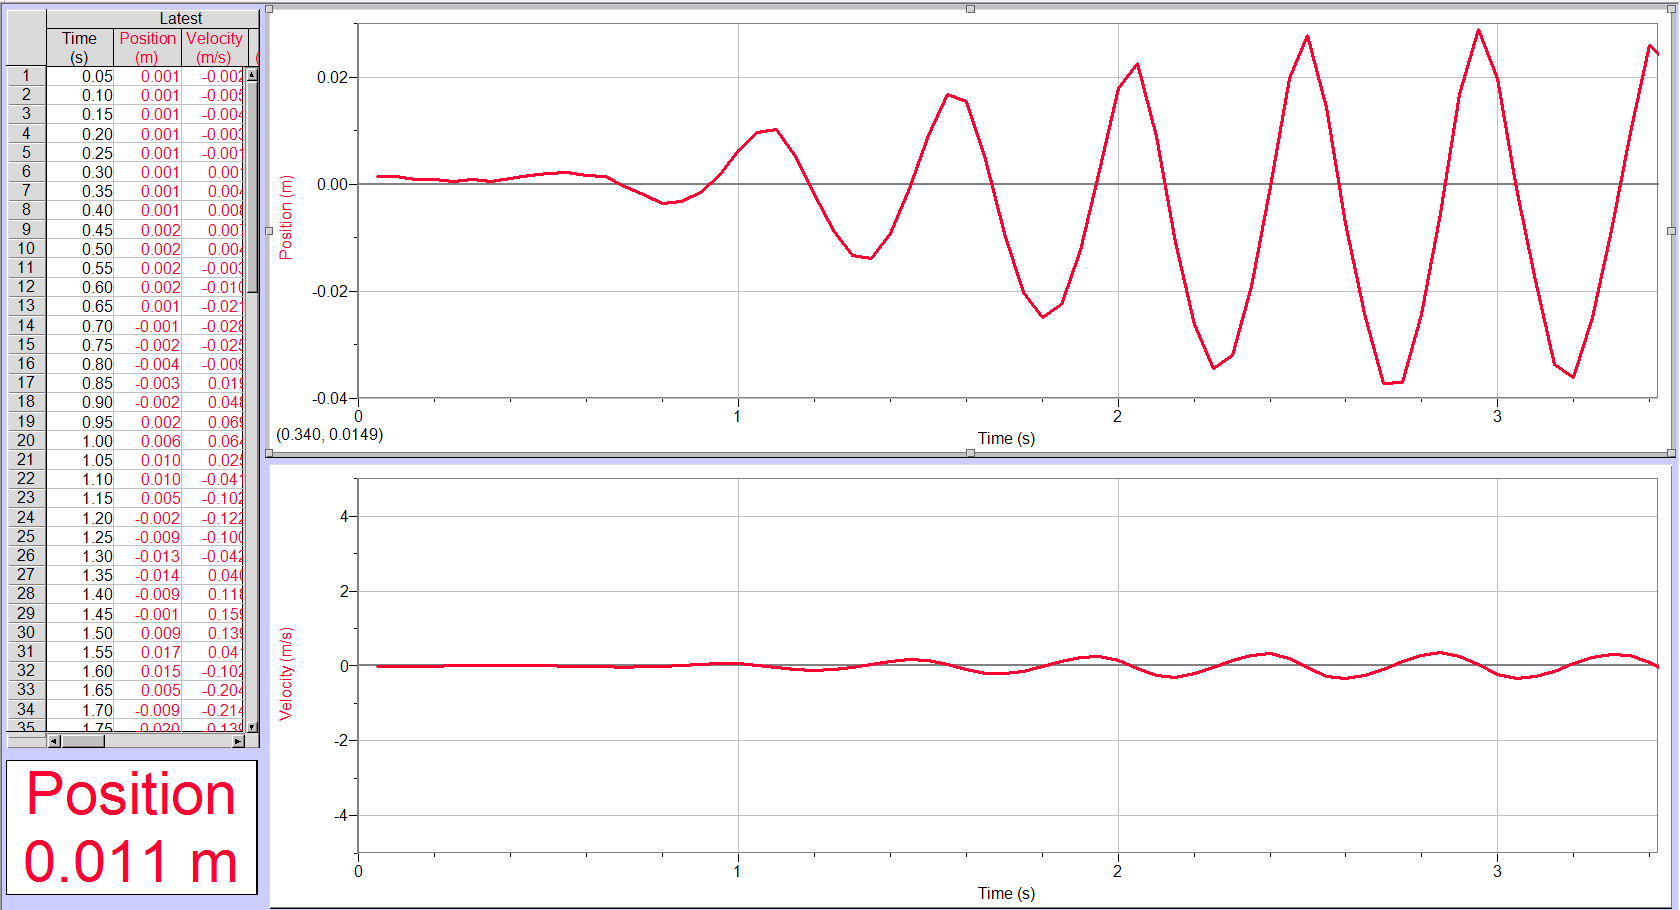
\includegraphics[width=\textwidth]{res/forced_undamped}
	\caption{Undamped Oscillation}
	\label{fig:Undamped Oscillation}
\end{figure}

\begin{figure}[H]
	\centering
	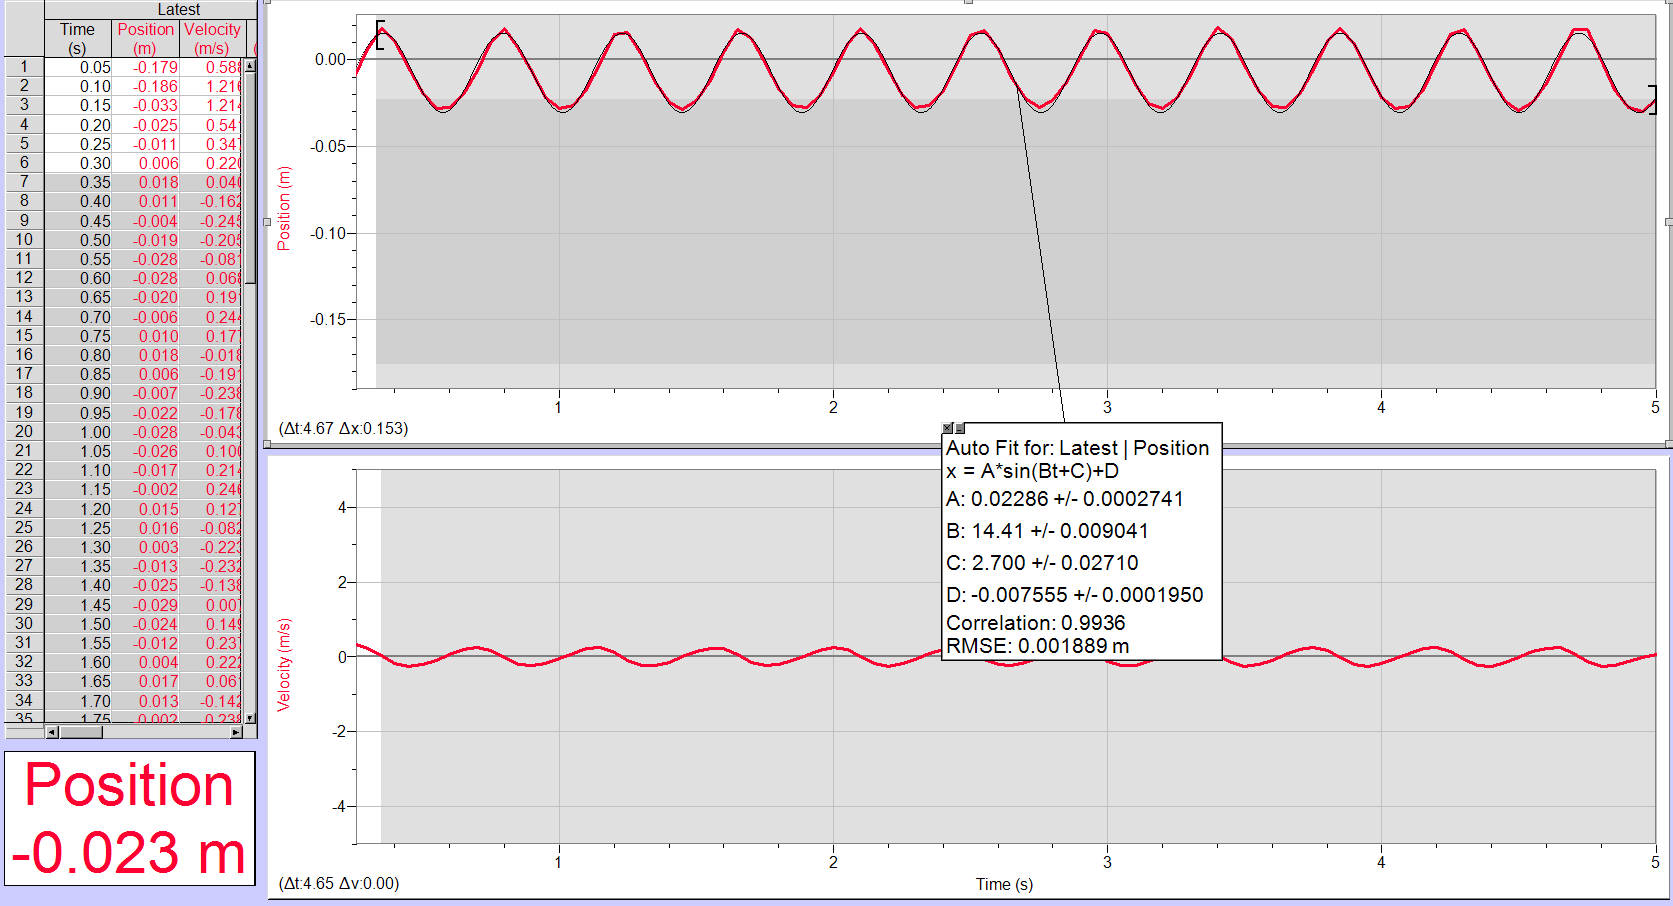
\includegraphics[width=\textwidth]{res/Damped}
	\caption{Damped Mass Oscillating}
	\label{fig:Damped Mass Oscillating}
\end{figure}


\begin{figure}[H]
	\centering
	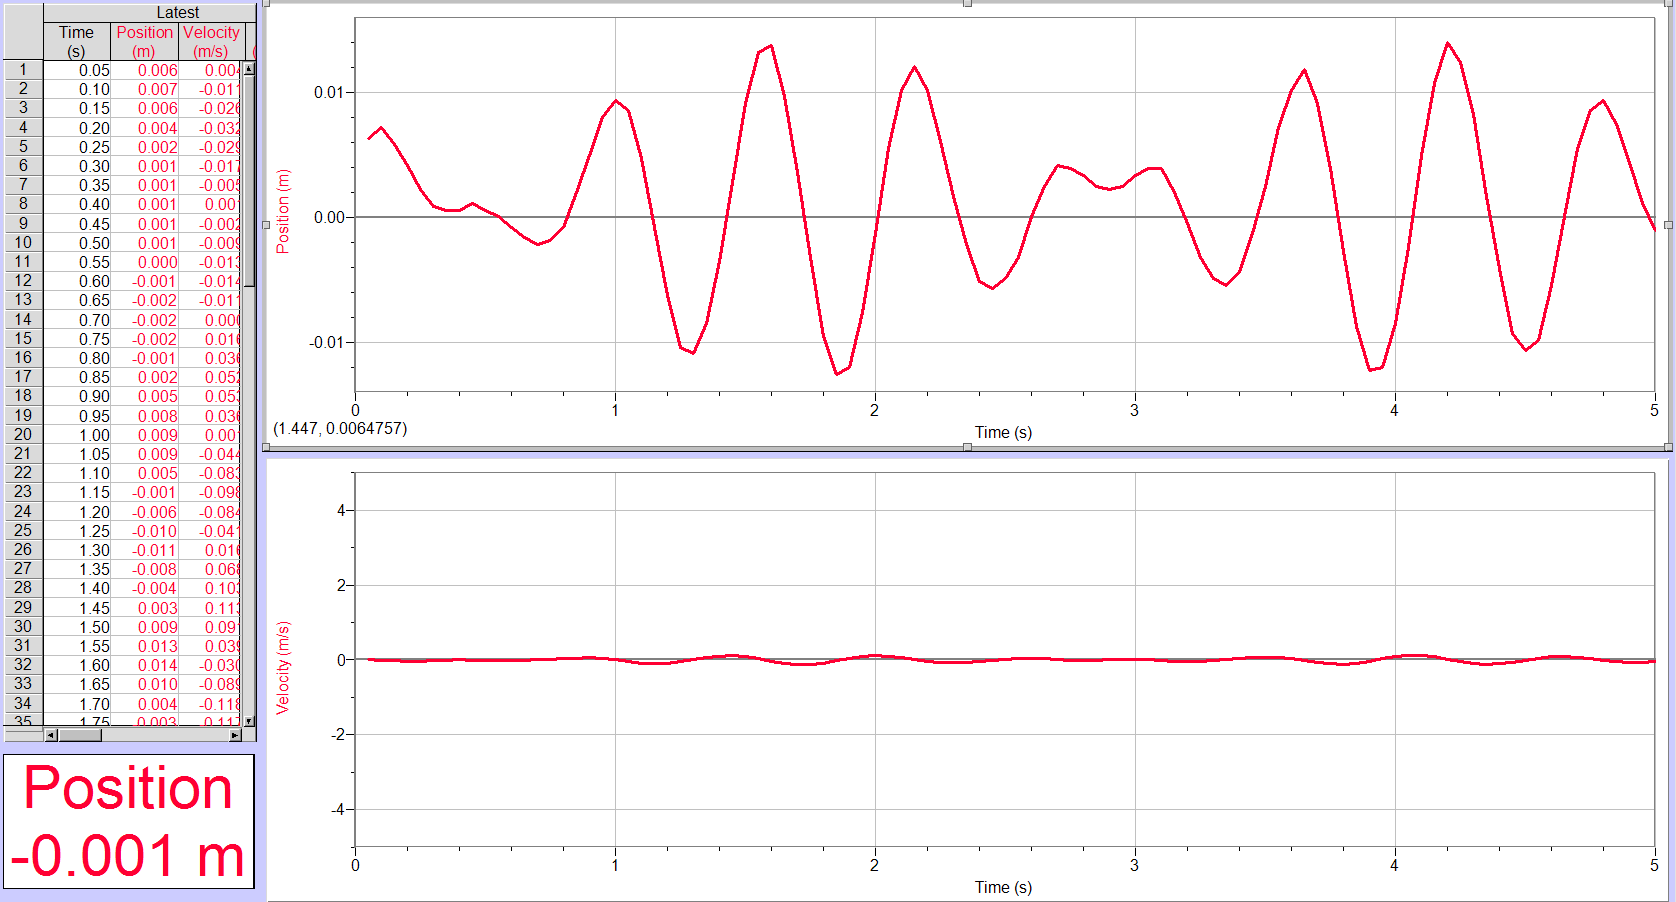
\includegraphics[width=\textwidth]{res/part3_1point5_hz}
	\caption{Mass with Medium Damper}
	\label{fig:Mass with Medium Damper}
\end{figure}




\section{Discussion}

In the Results section, we noticed that the undamped system reached its highest amplitude of 3 cm in 5 cycles. We can use these numbers to determine the average power delivered by the sine wave generator:

\begin{equation}
\begin{split}
	P&=\frac{w}{t}\\
	w&=\frac{1}{2}k*x^2	=\frac{1}{2}(16.22)0*.03^2	=.0073\\
	t&=5*T =5*\frac{1}{f} =5*\frac{1}{2} =2.5\\
	P&=\frac{w}{t} =\frac{.0073}{2.5} =.00292 J/s\\
\end{split}
\end{equation}

The Q factor must be significantly greater than $\frac{1}{2}$ because the system is very underdamped.



\end{document}          
